\subsection{Target dependence: a quadratic control}
\label{app:quadratic-control}

Replacing the mixed sine by $x^2$, normalized by its training-grid RMS,
tests whether the acquired slope scale depends on target content. We retain
width~512, five paired initializations, FP64 arithmetic, and the grids and
output-error criterion in Appendix~\ref{app:slope-experiments}.
Following the two-million-update rate search and a lower-rate Adam
expansion, one rate per optimizer and schedule is rerun from initialization
for five million updates. Cosine decay spans this full horizon. This
secondary control retains one rate per schedule, whereas the primary target
retains two. Final validation error selects one complete recipe per
optimizer by its median across the five seeds; no earlier checkpoint or
per-seed recipe replaces it. The 8,192-point grid checks resolution rather
than providing an untouched generalization test.

Adam selects cosine decay from $0.002$ and reaches median dense relative
error $5.434\times10^{-5}$; GD selects constant rate $0.1$ and reaches
$6.298\times10^{-4}$. Their median RMS values of $h|a_j|$ are $0.001357$
and $0.0005944$, and their median neuronwise $99$th percentiles are
$0.007401$ and $0.001503$, with $h=2/467$. This smoother target therefore
reaches lower error with substantially smaller slope statistics than the
mixed sine. The uniform-dictionary reference $1/4$ is not a universal
threshold for learned heterogeneous features.

\begin{figure}[t]
 \centering
 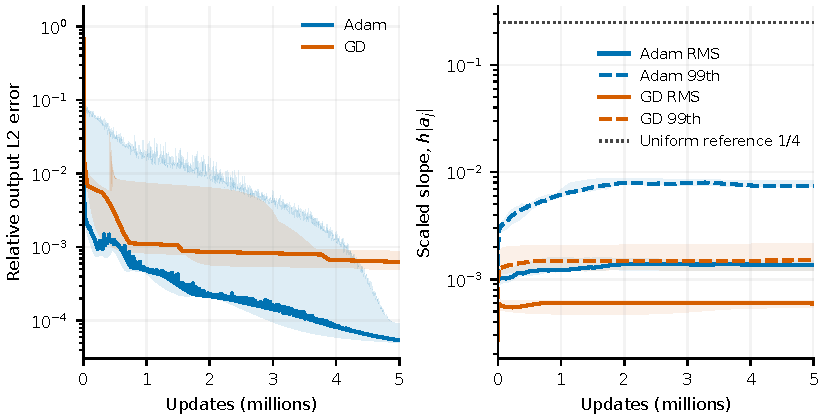
\includegraphics[width=\linewidth]{output/diagnostics/section34_long_horizon/quadratic/analysis_5m/joint_error_and_slopes.pdf}
 \caption{Quadratic joint training over five million updates, using five
 paired seeds. Left: raw relative training error, with median lines and
 shading retaining seed ranges and within-bin extrema. Right: RMS and
 neuronwise $99$th-percentile scaled slopes from the same runs; shading
 shows seed ranges and also preserves within-bin extrema for RMS. The
 dotted line is a uniform-dictionary reference, not a required slope for
 this target.}
 \label{fig:quadratic-joint}
\end{figure}

The longer horizon reduces Adam's median error from $1.633\times10^{-4}$
at two million updates, with all five seeds improving. Its trailing-window
median raw error still decreases by $35.7\%$ across the final fifth of the
five-million horizon, while the $99$th-percentile slope decreases by
$1.23\%$. Thus error improvement need not track a monotone increase in a
scalar slope statistic, and these finite-budget results do not establish
permanent training failure.

\paragraph{Separate frozen-dictionary checks at two million updates.}
At $\lambda=1/32,1/16,1/8,1/4$, the theorem lower bound divided by executed
GD error stays above $0.7633,0.7827,0.7852,0.7852$ at every update; its
endpoint ratios are $0.8453,0.9117,0.9324,0.9347$. The largest apparent
violation is $2.0\times10^{-15}$, and the exact-spectrum reference differs
from executed GD by at most $8.5\times10^{-15}$. Among uncensored tolerance
crossings, the necessary times are $62.4$--$88.0\%$ of executed times.
These are checked floating-point evaluations, not interval certificates.
The separate frozen Adam sweep reaches dense errors
$2.328\times10^{-4}$, $1.399\times10^{-4}$, and $5.985\times10^{-5}$ at
$\lambda=3/32,1/8,1/4$. Every selected recipe is at a boundary of the
expanded rate grid; these are best-in-grid outcomes, not optimizer optima.
Their two-million-update budget is kept separate from the joint figure.
